\documentclass{article}
\usepackage{amsmath}
\usepackage{hyperref}
\usepackage{graphicx}
\graphicspath{ {./data/results} }

\title{Option Pricing Strategy}
\author{Ayan Goswami}
\date{}
\begin{document}
\maketitle
\section{Introduction}

This document summarizes the findings reported in \texttt{strategy\_book.pdf}. The original analysis uses option data to evaluate pricing efficiency and develop a trading approach. A K--Nearest Neighbors (KNN) model is employed as a non-parametric estimator of conditional expectations $E(X\mid Y,Z,\ldots)$. The KNN output serves as a prior input in a Bayesian framework to signal long or short trades.

\section{Data Loading and Preparation}

Option data was loaded from a socket stream leveraging Alpaca's IEX market data (see ./socket), updated every 10 seconds. For the purposes of this investigation, we focused on options with 0 days to expiry (0dte), as they have the largest trading volume and are assumed to self-correct quicker than options with a later expiry. All options between 99\% to 101\% of the current price were stored in a csv, along with all the corresponding greeks and implied volatility. To read more about how this was calculated see the Appendix. When this investigation was conducted, SPY hovered around 620\$, hence for a given timestamp, 14 or 15 calls and puts were stored. This was done to get an even spread of in the money (ITM), at the money (ATM) and out the money (OTM) options.

Moneyness, defined as the relative position of the underlying asset price to the strike price, exhibits a strong relationship with the option premium. For call options, those that are in the money (ITM), i.e., with strike prices lower than the spot price (\(K < S\)), tend to have higher intrinsic value and thus higher premiums. Conversely, out of the money (OTM) options (\(K > S\)) carry mostly time value and are priced lower. This nonlinear relationship is especially pronounced in short-dated options, where the time decay is steep and the implied volatility surface varies across moneyness levels. Empirically, our dataset reflects this convex structure, with ATM options (\(K \approx S\)) typically exhibiting peak implied volatilities and forming the apex of the option price curve.

There is usually a very steep drop-off in 0dte OTM options' prices, mainly due to the fact that they will expire worthless by the end of the day. To enable fair comparison of option prices across different timestamps and mitigate scale differences between call and put options, we applied a logarithmic normalization procedure to standardize the prices. The transformation is defined as:

\[
\text{standardized\_price} = \frac{\log(p + 1) - \log(p_{\min} + 1)}{\log(p_{\max} + 1) - \log(p_{\min} + 1)}
\]

where \(p\) is the latest trade price of the option, and \(p_{\min}, p_{\max}\) are the minimum and maximum trade prices for a given option type (call or put) within a specific timestamp.

This transformation is applied separately for call and put options, and performed independently at each timestamp. The rationale is twofold: (1) call and put options have inherently different pricing distributions, and (2) the market conditions change across timestamps, requiring local normalization to preserve intra-timestamp price structure. 

Logarithmic scaling was chosen to compress the skewness in price distribution, especially in deep ITM or OTM options where price differences can be exponential. Adding 1 inside the logarithm avoids issues with near-zero prices. The result is a normalized feature \texttt{standardized\_price} bounded in \([0, 1]\), suitable for downstream tasks such as KNN modeling and residual analysis. The following is a random timestamp slice:
\begin{figure}[h]
  \centering
  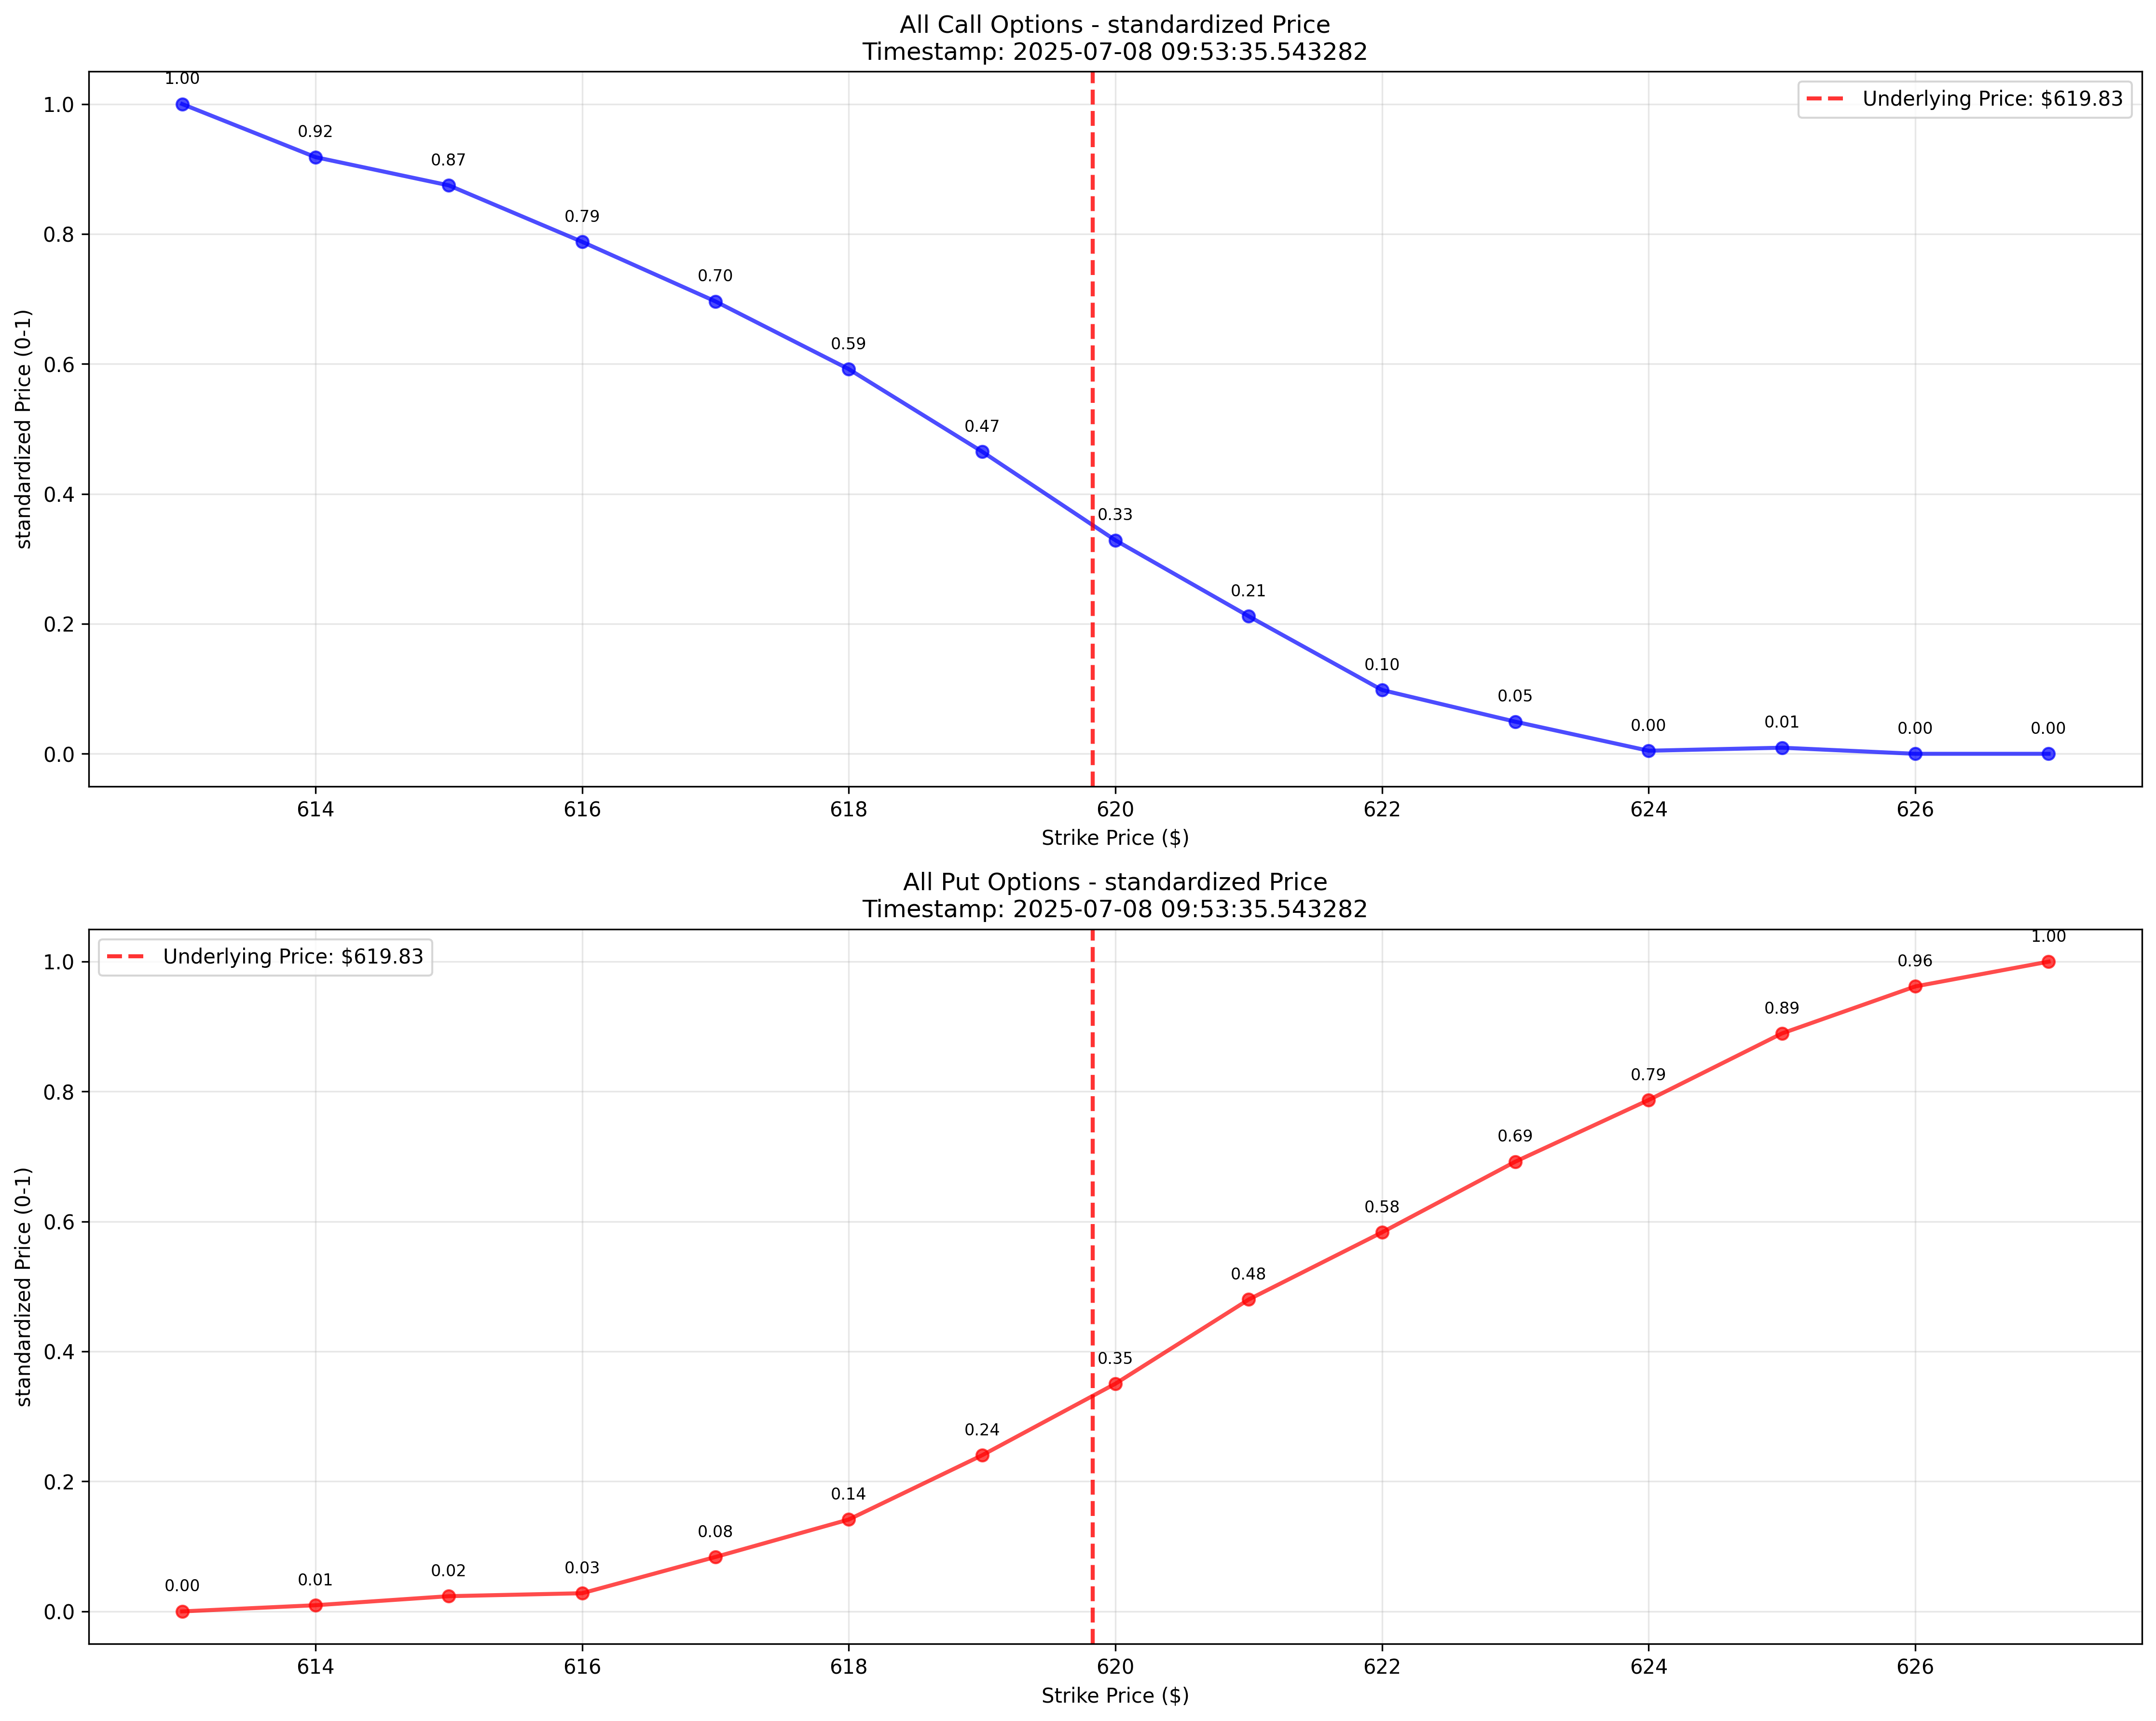
\includegraphics[width=0.8\linewidth]{calls_puts_timestamp_329}
  \caption{Standardized option prices for a given strike}
  \label{fig:price-std}
\end{figure}
\includegraphics{}

Option data were loaded from several processed files and split into training and validation sets using a 75\%/25\% split. Since the $\theta$ decay is so high for 0dte options, we focused on trade entry and exit windows between 30 seconds to 5 minutes. This way the $\alpha$ can be measured reliably without accounting for price decay. Hence, a column was appended to our dataset called \texttt{price\_diff}, which measured:
\[
\text{price\_diff_x} = \frac{\frac{\sum_{i=t}^{x+t}{price_i}}{x}}{price_{t}}
\]

where x is the look-forward period in tens of seconds, and t is the current time period. This will serve as a metric of success and efficacy in our paper.

\section{KNN Modeling}
The model predicts standardized option prices. A wrapper function scales predictors and returns both root mean squared error (RMSE) and $R^2$ values. Exhaustive subset selection determined that \verb|delta|, \verb|gamma|, \verb|moneyness|, and \verb|rho| gave the best performance with
\begin{align*}
\text{RMSE} &= 0.0269,\\
R^2 &= 0.9946.
\end{align*}
Optimal $k$ was found by evaluating a range of values and occurred at $k=3$. Residual analysis showed near-normal errors; a significance threshold was derived as
\begin{equation*}
q = \Phi^{-1}(0.95,\mu_{r},\sigma_{r}) = 0.0146,
\end{equation*}
where $r$ denotes prediction residuals.
\section{Hypothesis Testing}
Price moves were summarized by
\begin{equation*}
price\_diff_{x} = \frac{\frac{\sum_{i=t}^{t+x}{price_i}}{x}}{price_{t}}.
\end{equation*}
Mean returns were compared for options with residuals above $q$ (GEQ), below $-q$ (LEQ), and for all options. The null hypothesis
\begin{equation*}
H_0 : \mu_{\text{GEQ}} = \mu_{\text{LEQ}} = \mu_{\text{All}}
\end{equation*}
was rejected for the six-period window with p-values below 0.05. The alternative hypothesis
\begin{equation*}
H_1 : \mu_{\text{GEQ}} > \mu_{\text{All}} > \mu_{\text{LEQ}}
\end{equation*}
was supported in several horizons.
\section{Trading Simulation}
Signals were generated on new data using the KNN predictions. Long trades were entered when residuals exceeded $q$, and short trades were entered when residuals were less than $-q$. If $price\_diff\_x$ is the average future price ratio, then
\begin{align*}
\alpha_{\text{long}} &= (price_t \cdot price\_diff_x) - price_t,\\
\alpha_{\text{short}} &= price_t - (price_t \cdot price\_diff_x).
\end{align*}
A test run on 5268 trades produced \$1685 in profit. Comparison against 100 random simulations gave a null threshold of \$445.64, indicating the strategy outperformed chance at the five percent level.
\section{Results}
Figure~\ref{fig:price-diff} shows the average price change by residual group. The high residual group typically exhibits a higher mean price ratio across horizons. Table~\ref{tab:mean-return} lists mean future price ratios and $p$-values for each window.
\begin{figure}[h]
  \centering
  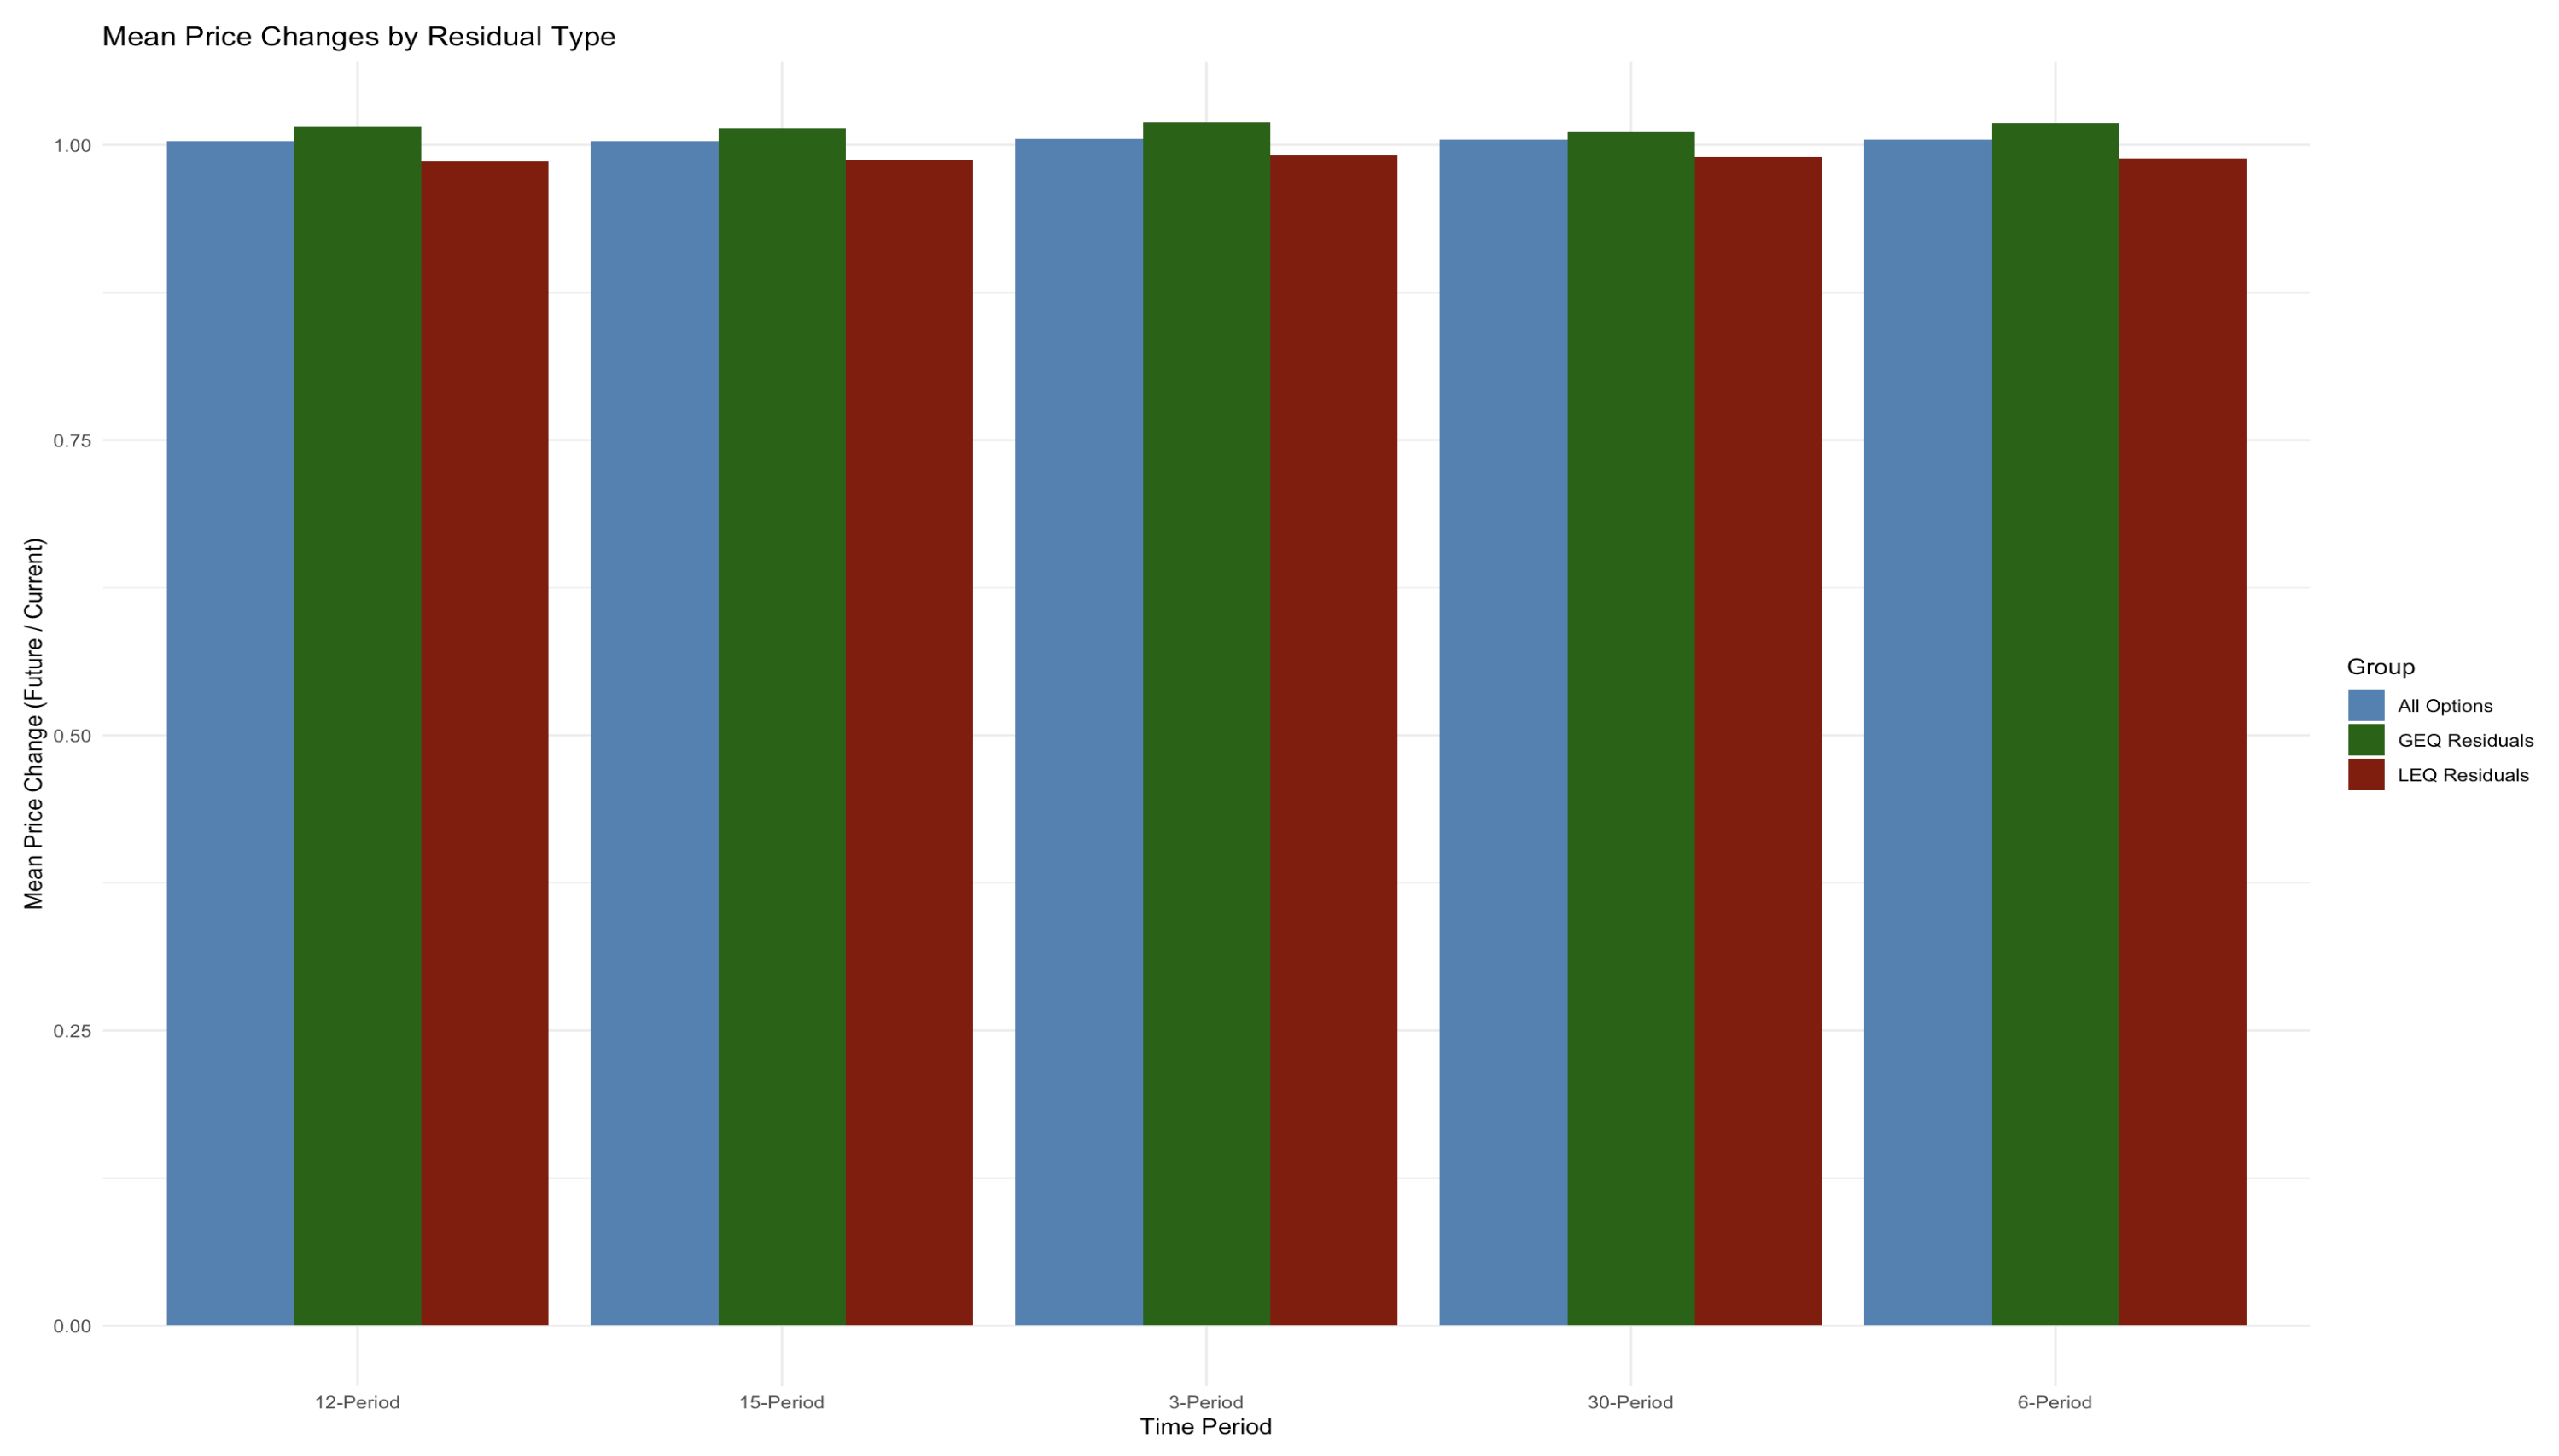
\includegraphics[width=0.8\linewidth]{data/results/mean_price_diff.png}
  \caption{Mean future price ratios by residual group}
  \label{fig:price-diff}
\end{figure}
\begin{table}[h]
  \centering
  \resizebox{\textwidth}{!}{%
    \begin{tabular}{lcccccc}
      \toprule
      Period (10s) & Mean (Under) & Mean (Over) & Mean (Overall) & $P(\mu_{\text{GEQ}} = \mu_{\text{All}})$ & $P(\mu_{\text{All}} = \mu_{\text{LEQ}})$ \\
      \midrule
      3   & 1.0111 & 0.9932 & 1.0019 & 0.0742   & 0*       \\
      6   & 1.0125 & 0.9915 & 0.9991 & 0.0265*  & 0.0006*  \\
      12  & 1.0114 & 0.9889 & 0.9989 & 0.0504   & 0.0003*  \\
      15  & 1.0086 & 0.9897 & 0.9975 & 0.0818   & 0.0052*  \\
      30  & 1.0028 & 0.9889 & 0.9961 & 0.2437   & 0.0405*  \\
      \bottomrule
    \end{tabular}%
  }
  \caption{Mean future price ratios by residual group and associated $p$-values. * indicates significance at $p = 0.05$.}
  \label{tab:mean-return}
\end{table}
\section{Discussion}
The KNN output served as a prior that highlighted relative mispricing. The residual-based signals produced consistent return differences in favor of positive residuals. While the profits observed in backtesting were modest, the approach performed better than random trading according to the null threshold. Further study could refine feature selection and risk controls.

Moreover, machine learning models such as random forests and boosted trees perform better than a naive Bayes solution such as this one according to Caruana (2006).
 
\section{Conclusion}
The KNN model approximates $E(X\mid Y,Z,\ldots)$ and acts as a prior in a Bayesian decision rule. Trades are triggered when observed residuals cross the significance threshold. The strategy generated profits above a random baseline, suggesting predictive value in the modeled relationships.

\appendix
\section{Black-Scholes Formulas}
\subsection{Option Pricing Formulas}
The Black-Scholes model for European option pricing is given by the following formulas:

\subsubsection{Call Option Price}
\begin{equation}
C(S, K, T, r, \sigma) = S \cdot N(d_1) - K e^{-rT} \cdot N(d_2)
\end{equation}

\subsubsection{Put Option Price}
\begin{equation}
P(S, K, T, r, \sigma) = K e^{-rT} \cdot N(-d_2) - S \cdot N(-d_1)
\end{equation}

\subsubsection{Parameters $d_1$ and $d_2$}
\begin{equation}
d_1 = \frac{\ln(S/K) + (r + \sigma^2/2)T}{\sigma\sqrt{T}}
\end{equation}

\begin{equation}
d_2 = d_1 - \sigma\sqrt{T}
\end{equation}

where:
\begin{itemize}
  \item $S$ = Current stock price
  \item $K$ = Strike price
  \item $T$ = Time to expiration (in years)
  \item $r$ = Risk-free interest rate
  \item $\sigma$ = Volatility of the underlying asset
  \item $N(\cdot)$ = Cumulative distribution function of the standard normal distribution
\end{itemize}

\subsection{Option Greeks}
The Greeks measure the sensitivity of option prices to various factors:

\subsubsection{Delta}
Measures the rate of change of option price with respect to changes in the underlying asset's price.

\textbf{Call Option Delta:}
\begin{equation}
\Delta_{call} = N(d_1)
\end{equation}

\textbf{Put Option Delta:}
\begin{equation}
\Delta_{put} = N(d_1) - 1
\end{equation}

\subsubsection{Gamma}
Measures the rate of change of delta with respect to changes in the underlying price.
\begin{equation}
\Gamma = \frac{N'(d_1)}{S\sigma\sqrt{T}} = \frac{e^{-\frac{d_1^2}{2}}}{S\sigma\sqrt{2\pi T}}
\end{equation}

Gamma is the same for both call and put options.

\subsubsection{Theta}
Measures the rate of change of option price with respect to the passage of time (time decay).

\textbf{Call Option Theta:}
\begin{equation}
\Theta_{call} = -\frac{S N'(d_1)\sigma}{2\sqrt{T}} - rKe^{-rT}N(d_2)
\end{equation}

\textbf{Put Option Theta:}
\begin{equation}
\Theta_{put} = -\frac{S N'(d_1)\sigma}{2\sqrt{T}} + rKe^{-rT}N(-d_2)
\end{equation}

Theta is typically expressed in value per day, dividing by 365.

\subsubsection{Vega}
Measures the rate of change of option price with respect to changes in volatility.
\begin{equation}
Vega = S\sqrt{T}N'(d_1)
\end{equation}

Vega is the same for both call and put options and is typically expressed as change per 1\% change in volatility.

\subsubsection{Rho}
Measures the rate of change of option price with respect to changes in the risk-free interest rate.

\textbf{Call Option Rho:}
\begin{equation}
\rho_{call} = KTe^{-rT}N(d_2)
\end{equation}

\textbf{Put Option Rho:}
\begin{equation}
\rho_{put} = -KTe^{-rT}N(-d_2)
\end{equation}

Rho is typically expressed as change per 1\% change in interest rate.

\subsection{Implied Volatility}
Implied volatility is the volatility value that, when input into the Black-Scholes formula, yields a theoretical option price equal to the market price. It is typically solved using numerical methods such as the Newton-Raphson method:

\begin{equation}
\sigma_{n+1} = \sigma_n - \frac{BS(S, K, T, r, \sigma_n) - Market\_Price}{Vega}
\end{equation}

where $BS(\cdot)$ is the Black-Scholes pricing function and iterations continue until convergence.

\subsection{Put-Call Parity}
For European options on non-dividend paying stocks:
\begin{equation}
C + Ke^{-rT} = P + S
\end{equation}

This relationship can be used to derive the price of a put option from a call option with the same strike and expiration, or vice versa.

\section{References}
1. Caruana, R.; Niculescu-Mizil, A. (2006). An empirical comparison of supervised learning algorithms. Proc. 23rd International Conference on Machine Learning.

\end{document}